% file: thermo.tex
% Thermodynamics, in unconventional ``grande'' format; fitting a widescreen format
% 
% If you liked this this file or found it useful, please consider donating on my Tilt/Open 
% campaign: I'd want to raise money for a new computer. 
% ernestyalumni.tilt.com 
%
% Facebook      : ernestyalumni 
% github        : ernestyalumni
% gmail         : ernestyalumni 
% linkedin      : ernestyalumni 
% twitter       : ernestyalumni 
% wordpress.com : ernestyalumni
% youtube       : ernestyalumni 
% Tilt/Open     : ernestyalumni
%
% This code is open-source, governed by the Creative Common license.  Use of this code is governed by the Caltech Honor Code: ``No member of the Caltech community shall take unfair advantage of any other member of the Caltech community.'' 
% 

\documentclass[10pt]{amsart}
\pdfoutput=1
\usepackage{mathtools,amssymb,lipsum,caption}

\usepackage{graphicx}
\usepackage{hyperref}
\usepackage[utf8]{inputenc}
\usepackage{listings}
\usepackage[table]{xcolor}
\usepackage{pdfpages}
\usepackage{tikz}
\usetikzlibrary{matrix,arrows}

\usepackage{multicol}

\hypersetup{colorlinks=true,citecolor=[rgb]{0,0.4,0}}

\oddsidemargin=15pt
\evensidemargin=5pt
\hoffset-45pt
\voffset-55pt
\topmargin=-4pt
\headsep=5pt
\textwidth=1120pt
\textheight=595pt
\paperwidth=1200pt
\paperheight=700pt
\footskip=40pt








\newtheorem{theorem}{Theorem}
\newtheorem{corollary}{Corollary}
%\newtheorem*{main}{Main Theorem}
\newtheorem{lemma}{Lemma}
\newtheorem{proposition}{Proposition}

\newtheorem{definition}{Definition}
\newtheorem{remark}{Remark}

\newenvironment{claim}[1]{\par\noindent\underline{Claim:}\space#1}{}
\newenvironment{claimproof}[1]{\par\noindent\underline{Proof:}\space#1}{\hfill $\blacksquare$}

%This defines a new command \questionhead which takes one argument and
%prints out Question #. with some space.
\newcommand{\questionhead}[1]
  {\bigskip\bigskip
   \noindent{\small\bf Question #1.}
   \bigskip}

\newcommand{\problemhead}[1]
  {
   \noindent{\small\bf Problem #1.}
   }

\newcommand{\exercisehead}[1]
  { \smallskip
   \noindent{\small\bf Exercise #1.}
  }

\newcommand{\solutionhead}[1]
  {
   \noindent{\small\bf Solution #1.}
   }


\title{Thermodynamics}
\author{Ernest Yeung \href{mailto:ernestyalumni@gmail.com}{ernestyalumni@gmail.com}}
\date{18 octobre 2015}
\keywords{Thermodynamics}
\begin{document}

\definecolor{darkgreen}{rgb}{0,0.4,0}
\lstset{language=Python,
 frame=bottomline,
 basicstyle=\scriptsize,
 identifierstyle=\color{blue},
 keywordstyle=\bfseries,
 commentstyle=\color{darkgreen},
 stringstyle=\color{red},
 }
%\lstlistoflistings

\maketitle

\tableofcontents

\begin{multicols*}{2}

\begin{abstract}
Everything about thermodynamics.  

I also look at thermodynamics for engineers from a (theoretical and mathematical) physicists' point of view.  I would like to seek more cross-polination between physicists and mathematicians and engineers in thermodynamics.
\end{abstract}

\part{Notes and Solutions for \emph{Thermal Physics} by Ralph Baierlein}\cite{RBaierlein1999}

\section{Background}

\subsection{Heating and Temperature}

Heating: keep in mind 3 different types of heating for energy exchange between two systems:

\begin{enumerate}
  \item Heating by conduction - literal contact, molecules jiggle faster from molecules jiggling faster by bouncing off them
  \item Heating by radiation - em waves from hot source strike and excite target
  \item heating by convection - energy transport by flow (perhaps a fluid)
\end{enumerate}

This all relates to \\
$Q$

\subsection{Some dilute gas relationships}

\subsubsection*{Pressure according to kinetic theory} i.e. some kinetic theory

$F \equiv $ force on area $A$ due to molecules \\
$\Delta p \equiv $ momentum transferred to wall per collision \\
$n \equiv$ number of collisions in time $\Delta t$

Thus
\[
F = \frac{ (\Delta p)n }{ \Delta t }
\]

Now $\Delta p = 2 m v_x$ since $\Delta p = mv_x - (-mv_x) = 2mv_x$ (elastic collision with momentum conversation)

$v_x \Delta t A$ is a volume, inside of which gas molecules can be within distance $v_x \Delta t$ toward the wall.  \\
$\frac{N}{V}$ number density of molecules

Assume equal distribution of velocities: Thus $\frac{1}{2}$
\[
 n = (v_x \Delta t A) \frac{1}{2} \frac{N}{V}
\]
\[
P = \frac{F}{A} = \frac{ (2mv_x)(v_x \Delta t A ) \frac{1}{2} \frac{N}{V} }{ A \Delta t} = mv_x^2 \frac{N}{V}
\]

Suppose $\langle v^2 \rangle = \langle v_x^2 \rangle + \langle v_y^2 \rangle + \langle v_z^2 \rangle = 3 \langle v_x^2 \rangle = d \langle v_x^2 \rangle$.  
\[
\Longrightarrow P = \frac{mN}{dV} \langle v^2 \rangle = \frac{2}{d} \frac{1}{2} m \langle v^2 \rangle \frac{N}{V}
\]

\subsubsection*{An empirical gas law}
Now 
\[
P = \frac{N\tau}{V} \quad \, \text{(empirical)}
\]

\[
\Longrightarrow \frac{1}{2} m \langle v^2 \rangle = \frac{d}{2} \tau
\]

\subsection{The First Law of Thermodynamics}

\[
dU = Q - W \text{ or } Q = dU + W 
\]

Consider $W = Q-dU$.  

Consider path in $M$, $\gamma$, $\begin{aligned} & \quad \\
  & \gamma : \mathbb{R} \to M = (U,V) \\
  & \gamma(t) = (U(t), V(t)) \end{aligned}$

$\dot{\gamma} \in \mathfrak{X}(M)$, $\dot{\gamma} = \dot{U} \frac{\partial }{ \partial U} + \dot{V} \frac{ \partial }{ \partial V}$

\[
W(\dot{\gamma}) = pdV(\dot{\gamma}) = p\dot{V} = Q(\dot{\gamma}) - dU(\dot{\gamma}) = Q(\dot{\gamma}) - \dot{U}
\]
Suppose $Q(\dot{\gamma}) = Q(t)dt(\dot{\gamma} \frac{ \partial }{ \partial t} ) = Q(t) \dot{\gamma}$.  
\[
\begin{gathered}
  \int p \dot{V} dt = \int Q(t) \dot{\gamma}dt - \int \dot{U}dt \\ 
  \Longrightarrow p\Delta V = \Delta Q - \Delta U
\end{gathered}
\]
$p\Delta V$ interpreted as work done by gas. $\Delta Q$ is heat transferred to gas system.  $-\Delta U$ is the drop in internal energy of gas system as it does work.  

\subsection{Heat capacity}

\[
Q = Q(\tau,V) = \left( \frac{ \partial Q}{ \partial \tau} \right)_V d\tau +  \left( \frac{ \partial Q}{ \partial V} \right)_{\tau} dV
\]
So define $C_V \equiv \left( \frac{ \partial Q}{ \partial \tau} \right)_V$ or interpret $C_V$ as energy input by heating at constant volume over ensuing change in temperature.  

In this case, $\left( \frac{ \partial U}{ \partial \tau } \right)_V$.  

For the case of a monatomic gas, $U =\frac{d}{2} \tau N$, $\frac{ \partial U}{ \partial \tau} = \frac{d}{2} N$.  
\[
C_V = \frac{d}{2} N
\]
$N \equiv $ number of molecules.  

Now 
\[
\begin{aligned}
  & Q = \Lambda_p dp + C_p d\tau \\ 
  & Q = \Lambda_V dV + C_V d\tau
\end{aligned} \Longrightarrow \begin{aligned}
  & Q \wedge dp = C_p d\tau \wedge dp \\ 
  & Q \wedge dp = \Lambda_V dV \wedge dp + C_V d\tau \wedge dp
\end{aligned}
\]
Now from the thermodynamic identity, $Q = W + dU = pdV + dU$,
\[
Q \wedge dp = p dV \wedge dp + dU \wedge dp
\]
and from (empirical) ideal gas law, $pV = N\tau$ (which defines a hypersurface on $M$),
\[
dp V + p dV = N d\tau \Longrightarrow p dV \wedge dp = N d\tau \wedge dp
\]
so then
\[
Q \wedge dp = N d\tau \wedge dp + dU \wedge dp
\]
In the case of the monatomic gas, $U = \frac{d}{2} \tau N$, and so $dU = \frac{d}{2} N d\tau = C_V d\tau$ and so comparing all the equations above, one recovers
\[
C_p = N + C_V = \frac{2+d}{2} N
\]
EY: 20151019 I'm curious to know how this all generalizes for $C_V$, $C_P$ heat capacities, regardless of the type of molecule we consider.  


\subsubsection*{The adiabatic relation for a classical ideal gas}

Consider the adiabatic expansion (or contraction!) of a classical ideal gas.  \\
This means that $Q=0$; there is no heat exchange to or from the gas system.  

Recall $Q = dU + W$.  \\
If $Q=0$, and supposing $W = pdV$, then $0 = dU + pdV$.  

EY : 20151019 Either by definition, or the thermodynamic identity, $\tau d\sigma = dU + pdV$, then $C_V := \left( \frac{ \partial U}{ \partial \tau} \right)_V$.  My question is this: for manifold of thermodynamic states $M$, $M=(U,V)$, i.e. $U$ is a global coordinate and $V$ is a ``local'' coordinate.  One can make a Legendre transformation such that $M$ is parametrized by $(\tau,V)$, where $\tau$ is the temperature.  In general, one should say that $U=U(\tau,V) \in C^{\infty}(M)$, and so $dU = \frac{ \partial U }{ \partial \tau} d\tau + \frac{ \partial U}{ \partial V} dV$, $dU \in \Omega^1(M)$.    

However, for this adiabatic process, we want
\[
Q = 0 = dU + W = dU + pdV = C_V d\tau + pdV
\]
which implies that $dU = C_V d\tau$.  What happened to the $\frac{ \partial U}{ \partial V} dV$? Is it that in this adiabatic process, the internal energy of the gas system goes to either doing work (expansion) or increases due to work being done on it (contraction), and is characterized completely by a drop or increase in its temperature, respectively?  And so $dU = C_V \tau$, and $pdV$ completely describes what's going on with work done or work done on it?

Nevertheless, using the (empirical) ideal gas law, $pV = N\tau$, 
\[
0 = C_V d\tau + pdV = C_V d\tau + \frac{N\tau}{V} dV
\]
Consider a path $\begin{aligned} & \quad \\
  & \gamma : \mathbb{R} \to M \\ 
  & \gamma(t) = (\tau(t), V(t)) \end{aligned}$ \quad \, in $M$, so that $\dot{\gamma}(t) = \dot{\tau} \frac{ \partial }{ \partial \tau } + \dot{V} \frac{ \partial }{ \partial V} \in \mathfrak{X}(M)$.  

Thus, 
\[
\begin{gathered}
  0 = C_v \dot{\tau} + \frac{N \tau}{V} \dot{V} \text{ so } \frac{ \dot{\tau}}{\tau} + \frac{N}{C_V} \frac{ \dot{V}}{V} \\
  \xrightarrow{ \int dt } \ln{ \frac{ \tau_f}{ \tau_i } } + \frac{N}{C_V} \ln{ \frac{V_f}{ V_i } } = 0 \text{ or } \ln{\tau V^{\frac{N}{C_V}} } = \text{ const. }
\end{gathered}
\]

Now
\[
\frac{N}{C_V} = \frac{C_P - C_V}{ C_V} = \gamma -1 
\]
which is true, assuming the (empirical) ideal gas law, the thermodynamic identity, and, surely, for the case of a monatomic gas.  

Thus
\[
\tau_f V_f^{\gamma-1} = \tau_i V_i^{\gamma -1}
\]

\subsection*{Problems}

\problemhead{4} \emph{Adiabatic compression}. 

A diesel engine doesn't have a spark plug to ignite and explode the fuel.  Instead, the air in the cylinder is compressed so highly that the fuel ignites spontaneously when sprayed into the cylinder.  

\begin{enumerate}
\item[(a)] 
\[
\begin{gathered}
  \frac{ \tau_f V_f^{\gamma -1} }{ \tau_i V_i^{\gamma -1} } = \frac{ P_f V_f^{\gamma }}{ P_i V_i^{\gamma} } = 1 \\
  \tau_f = \left( \frac{V_i}{V_f} \right)^{\gamma -1 }\tau_i
\end{gathered}
\]

Run the Python script \verb|thermo.py| to do the calculations.  Here is (some of) the code from \verb|thermo.py| for doing so (one still needs to import the necessary libraries):

\begin{lstlisting}
roomtemp_K = KCconv.subs(T_C,20).rhs # room temperature in Kelvin                               

Prob0104ans = adia_tV.subs(gamma,1.4).subs(V_f,1).subs(V_i,15).subs(tau_i, roomtemp_K) # answer to Problem 4 of Chapter 1                                                                           

Prob0104ans = N( Prob0104ans.lhs) # 866.016969686253 K                                         
Prob0104ansC = solve( KCconv.subs( T_K, Prob0104ans), T_C )[0] # 592.866969686253 C            
solve( FCconv.subs( T_C, Prob0104ansC ), T_F)[0] # 1099.16054543526 F   
\end{lstlisting}

The final temperature is $866.01 \, K$ or $592.87 \, C$ or $1099.16 \, F$

\item[(b)] Now from the ideal gas law, which is obeyed at all thermodynamic states
\[
\begin{gathered}
  \frac{P_f}{ P_i} = \frac{V_i}{V_f} \frac{ \tau_f}{ \tau_i}
\end{gathered}
\]
and so $\frac{P_f}{P_i} = 44.31$
\end{enumerate}


\section{Phase Equilibrium}

\subsection{Latent heat}

$p,T$ const., liquid $\to $ gas, e.g. $ \begin{aligned} & \quad \\
  & p = 1 \text{ atm } \\
  & T = 373 \, K \end{aligned}$

latent heat of vaporization $L_{\text{vap}}$ (by def.) amount of energy supplied by heating.  \\
$Q = dU + W$ \\
$\epsilon := U/N = $ average (internal) energy per molecule  \\
$v:= V/N = $ volume per molecule 

$L_{\text{vap}} = d\epsilon + p dV$ \\
\phantom{\quad \, } $d\epsilon(\dot{\gamma}) = \epsilon_{\text{vap}} - \epsilon_{\text{liq}}$ \\
\phantom{\quad \, } $dv(\dot{\gamma}) = v_{\text{vap}} - v_{\text{liq}} >0$

if $p$ const., $L_{\text{vap}} = d(\epsilon + pV) = dh$, $h:= H/N = \frac{ U + pV}{N}$

EY : 20151031 A better way to think about it is this: recall that
\[
\begin{aligned}
  & Q = dU + W = dU + pdV = \tau d\sigma \\ 
  & H = U + pV \text{ so } dH = dU + pdV + Vdp = Q + Vdp
\end{aligned}
\]
Consider a path $\gamma \in M$ s.t. $\begin{aligned} & \quad \\
  & d\tau(\dot{\gamma}) = 0 \\
  & dp(\dot{\gamma}) = 0 \end{aligned}$ \quad \, (constant $\tau,p$)

\[
\begin{aligned}
  & Q(\dot{\gamma}) = dH(\dot{\gamma}) - Vdp(\dot{\gamma}) = dH(\dot{\gamma}) - 0 = dH(\dot{\gamma})
  & Q(\dot{\gamma}) = \tau d\sigma(\dot{\gamma}) \\ 
  & \int Q(\dot{\gamma}) = \int \tau d\sigma(\dot{\gamma}) = \tau(\sigma_g - \sigma_l)
\end{aligned}
\]
Thus
\[
\begin{gathered}
  \frac{ \int Q(\dot{\gamma})}{ N} = \tau (s_g - s_l ) = \frac{H_g}{N} - \frac{H_l}{N} \\ 
  L \equiv \tau(s_g - s_l) = \frac{ \int Q(\dot{\gamma})}{ N} = \frac{1}{N} (H_g -H_l)
\end{gathered}
\]

\subsubsection*{Latent heat versus heat capacity}

Take slow, reversible process.  

Now 
\[
\begin{aligned}
  & C_V := \tau \left( \frac{ \partial \sigma }{ \partial \tau} \right)_V \\ 
  & C_P := \tau \left( \frac{ \partial \sigma }{ \partial \tau } \right)_P
\end{aligned}
\]

It's stated in Kittel and Kroemer (1980), pp. 166, Equation (37), Chapter 6: Ideal Gas, Subsection ``Heat capacity'' \cite{CKittelHKroemer1980}, that 
\begin{equation}
  C_P = \tau \left( \frac{ \partial \sigma }{ \partial \tau} \right)_P = \left( \frac{ \partial U }{ \partial \tau} \right)_P + p \left( \frac{ \partial V}{ \partial \tau} \right)_p
\end{equation}

Suppose $\sigma = \sigma(\tau, V)$.  With $\tau d\sigma = dU + W = \tau d\sigma = dU + pdV$, 
\[
\begin{aligned}
  & d\sigma = \frac{ \partial \sigma }{ \partial \tau } d\tau + \frac{ \partial \sigma }{ \partial V} dV = \frac{dU}{ \tau} + \frac{p}{\tau} dV \\ 
  & d\sigma(\dot{\gamma}) = \left( \frac{ \partial \sigma}{ \partial \tau} \right)_V + 0 = \frac{1}{\tau} dU(\dot{\gamma}) = \frac{1}{\tau} \left( \frac{ \partial U}{ \partial \tau} \right)_V
\end{aligned}
\]
Then it's clear that 
\[
\tau \left( \frac{ \partial \sigma }{ \partial \tau } \right)_V = \left( \frac{ \partial U}{ \partial \tau} \right)_V = C_V
\]

Now suppose $\sigma = \sigma(\tau, p)$.  

Consider also the enthalpy,  $H = U + pV$, and so
\[
dH = dU + Vdp + pdV = \tau d\sigma + Vdp
\]
Now for $\sigma = \sigma(\tau,p)$,
\[
\begin{aligned}
  & \sigma = \sigma(\tau,p) \\ 
  & d\sigma = \frac{ \partial \sigma }{ \partial \tau} d\tau + \frac{ \partial \sigma }{ \partial p } dp = \frac{dH}{\tau} - \frac{V}{\tau} dp
\end{aligned} \Longrightarrow d\sigma(\dot{\gamma}) = \left( \frac{ \partial \sigma }{ \partial \tau} \right)_p + 0 = \frac{1}{\tau} \left( \frac{ \partial H}{ \partial \tau} \right)_p - 0 
\]

So 
\[
C_p := \tau \left( \frac{ \partial \sigma }{ \partial \tau } \right)_p = \left( \frac{ \partial H}{ \partial \tau} \right)_p
\]
Now 
\[
\begin{gathered}
  dH(\dot{\gamma}) = dU(\dot{\gamma}) + Vdp(\dot{\gamma} ) + pdV(\dot{\gamma}) = \left( \frac{ \partial U }{ \partial \tau} \right)_p + 0 + p \left( \frac{ \partial V}{ \partial \tau} \right)_p = \left( \frac{ \partial H }{ \partial \tau } \right)_p \text{ so } \\ 
  C_p = \tau \left( \frac{ \partial \sigma }{ \partial \tau} \right)_p = \left( \frac{ \partial U}{ \partial \tau} \right)_p + p\left( \frac{ \partial V}{ \partial \tau} \right)_p 
\end{gathered}
\]

Kittel and Kroemer (1980) \cite{CKittelHKroemer1980} argues that for ideal gas, 
\[
\left( \frac{ \partial U}{ \partial \tau} \right)_p = \left( \frac{ \partial U}{ \partial \tau} \right)_V
\]
since $U = U(\tau)$.  

\subsection{Conditions for coexistence} Sec. 12.3 of Baierlein (1999) \cite{RBaierlein1999}.  

Recall 
\[
G = F + pV = U + pV - \tau \sigma =G(\tau,p,N)
\]

Now 
\[
\begin{gathered}
  G = G(\tau, p, N_{\text{vap}}, N_{\text{liq}} )
\Longrightarrow dG = \frac{ \partial G}{ \partial N_{\text{vap}}} dN_{\text{vap}} + \frac{ \partial G}{ \partial N_{\text{liq}} } dN_{\text{liq}} = \mu_{\text{vap}} 1 + \mu_{\text{liq}} (-1) = 0  \\
\Longrightarrow \mu_{\text{vap}}(\tau,p) = \mu_{\text{liq}}(\tau,p)
\end{gathered}
\]

From Kittel and Kroemer (1980) \cite{CKittelHKroemer1980}, Example : $N$ atoms in a box, Chapter 3: ``Boltzmann Distribution and Helmholtz Free Energy'', 

state of energy $\epsilon_{\alpha}(1) + \epsilon_{\beta}(2) + \dots + \epsilon_{\xi}(N)$, $\alpha, \beta, \dots \xi$ denote orbital indces of atoms in successive boxes.  \\
each entry occurs $N!$ times in $Z_1^N$ (EY: 20151022) $N!$ ways to fill $\alpha, \beta \dots \xi$ orbitals with $N$ distinguishable particles.  Thus,
\[
Z_N = \frac{1}{N!} Z_1^N = \frac{1}{N!} (n_Q V)^N
\]


\part{Notes and Solutions on \emph{Fundamentals of Thermodynamics}, 8th Edition, by Claus Borgnakke, Richard E. Sonntag}
\cite{CBorgnakkeRSonntag2012}

\section{}

\section{Properties of a Pure Substance}

EY : 20151030 Is the word vapor the same as gas?  vapour, gaz, gas, vapore

For coexistence equilibrium, 
\[
\begin{aligned}
  & \mu_g(p_0,\tau_0) = \mu_l(p_0,\tau_0) \text{ and } \\ 
  & \mu_g(p_0 + dp, \tau_0+d\tau) = \mu_l(p_0 + dp, \tau_0+d\tau)
\end{aligned}
\]
and so 
\begin{equation}
  \frac{dp}{d\tau} = \frac{L}{\tau \Delta v}
\end{equation}
where $v\equiv \frac{V}{N}$, the so-called \textbf{vapor pressure equation} or \textbf{Clausius-Clapeyron} equation.  

For (2) approximations, $\Delta v = v_g - v_l \approx v_g = \frac{V_g}{N_g}$ and idealize vapor as ideal gas, $pV = N\tau$ so $\frac{dp}{d\tau} = \frac{L}{\tau^2/p}$.  

Second, if $L$ constant, 
\begin{equation}\label{Eq:CCeq_pvsT}
  p(\tau) = p_0 \exp{ (-L_0/\tau)} \text{ or } \ln{ \left( \frac{p(\tau)}{p_0} \right) } = \frac{-L_0}{\tau}
\end{equation}
cf. Ch. 10 Phase Transformations, pp. 278-284, ``Derivation of the Coexistence Curve, $p$ Versus $\tau$'' of Kittel and Kroemer (1980) \cite{CKittelHKroemer1980}.  

Eq. \ref{Eq:CCeq_pvsT} explains the shape of the coexistence curve between solid and gas (vapor) (sublimation) and liquid and gas (vapor) (vaporization; vaporization curve).  

\textbf{Saturation} is this $p=p(\tau)$ coexistence curve.  


\textbf{Isotherms, Isothermals}

Recall $\begin{aligned} 
  & \quad \\
  & G = F + pV \\
  & F = U-\tau \sigma \end{aligned}$ and so $\begin{aligned}
  & \quad \\
  & dG = dF + Vdp + pdV = dU - \tau d\sigma - \sigma d\tau + pdV + Vdp = -\sigma d\tau + Vdp \\
  & dG = -\sigma d\tau + Vdp \end{aligned}$

So then $\begin{aligned} & \quad \\
  & G = G(\tau, p) \\
  & G= G(\tau, p, N) \end{aligned}$ 

where the latter statement is when we include particle transfer, so that 
\[
dG = -\sigma d\tau + Vdp + \mu dN \text{ for } \mu = \mu(\tau,p)
\]

For the \emph{ideal gas}:

\[
\begin{gathered}
  F(\tau,V) = F= -N\tau \left( \ln{ \left( \frac{n_Q}{n} \right)} + 1 \right) \\ 
  \text{ where }  \begin{aligned}
    & n_Q = \left( \frac{M\tau }{2\pi \hbar^2 } \right)^{3/2} \\ 
    & n \equiv N/V = \frac{p}{\tau} 
  \end{aligned} \\
  G(\tau,p, N) = -N \tau ( \ln{ \left( \frac{n_Q}{n} \right) } + 1 ) + N \tau = - N\tau ( \ln{ \left( \frac{n_Q}{n} \right) } ) = -N\tau \ln{ \left( \left( \frac{M\tau}{2\pi \hbar^2 } \right)^{3/2} \frac{\tau}{p} \right) } \\
  \text{ so then }
\left( \frac{ \partial G}{ \partial N} \right)_{\tau,p} = \mu = -\tau \ln{ \left( \left( \frac{M\tau}{2\pi \hbar^2} \right)^{3/2} \frac{\tau}{p} \right) }
\end{gathered}
\]

For the \emph{Van der Waals gas}
\[
\begin{gathered}
  F(vdW) = -N\tau \left( \ln{ \left( \frac{n_Q (V-Nb)}{N} \right) }  + 1 \right) - \frac{N^2 a }{V} \\ 
  p = -\left( \frac{\partial F}{ \partial V} \right)_{\tau,N} = \frac{N\tau}{V-Nb} - \frac{N^2a}{V^2} \\
  G(\tau,V,N) = \frac{N\tau V}{ V-Nb} - \frac{2N^2 a}{V} - N\tau ( \ln{ \left( \frac{n_Q (V-Nb)}{N} \right) } + 1 )
\end{gathered}
\]

Nevertheless, consider, when considering isotherms, isothermals, 
\[
dG = -\sigma d\tau  + Vdp + \mu dN
\]
Consider a path $\gamma$ on constant $\tau$, constant total number of particles $N$, and so
\[
dG(\dot{\gamma}) = Vdp(\dot{\gamma}) = G_g-G_l = \int_{\gamma} Vdp
\]


\part{Thermodynamics (Revisited)}

\section{Heat Capacity}

From Kittel and Kroemer (1980) \cite{CKittelHKroemer1980}, pp. 165-166, Chapter 6: Ideal Gas, ``Heat Capacity'',
\[
Q = Q(\tau,p) = \Lambda_p dp + C_p d\tau = dU + W = dU + p dV 
\]
Let $c\in \Sigma$ s.t. $dp(\dot{c})=0$ (constant pressure).  And so 
\[
Q(\dot{c}) = 0 + C_p d\tau(\dot{c}) = \tau d\sigma (\dot{c}) = dU(\dot{c}) + pdV(\dot{c})
\]
for $c=(\tau,0)$, $\dot{c} = \frac{\partial }{ \partial \tau} \in T\Sigma$.  

\[
\Longrightarrow C_p = \tau \left( \frac{ \partial \sigma }{ \partial \tau} \right)_p = \left( \frac{ \partial U}{ \partial \tau} \right)_p + p \left( \frac{ \partial V}{ \partial \tau} \right)_p
\]
for heat capacity at constant pressure is larger than $C_V$ because additional heat must be added to perform the work needed to expand volume of gas against constant pressure.  

Now recall for enthalpy 
\[
\begin{aligned}
  & H = U+ pV \\ 
  & H = H(\sigma, p)
\end{aligned}
\]
Then
\[
dH = dU+ pdV + Vdp = Q + Vdp 
\]
Thus, for $c\in \Sigma$, $dp(\dot{c})=0$ (constant pressure).  Hence
\[
dH(\dot{c}) = \left( \frac{ \partial H}{ \partial \tau} \right)_p = Q(\dot{c})  +  0 = C_p
\]
Hence, 
\[
C_p = \left( \frac{ \partial H}{ \partial \tau } \right)_p = \left( \frac{ \partial Q}{ \partial \tau} \right)_p
\]



\section{Phase Equilibrium}


\begin{description}
\item Phase Equilibrium
\item Phase Diagram
\item (Phase) Coexistence Curve 
\item Antoine Equation (parameters)
\end{description}


For coexistence equilibrium, $\mu_g(p_0,\tau_0) = \mu_l(p_0,\tau_0)$ and $\mu_g(p_0 + dp, \tau_0 + d\tau) = \mu_l(p_0 + dp, \tau_0+d\tau)$, and so $\frac{dp}{d\tau} = \frac{L}{ \tau \Delta v}$ with $v \equiv \frac{V}{N}$.  

Make the approximation that $\Delta v \equiv v_g - v_l \approx v_g = \frac{V_g}{N_g}$ and idealize vapor as ideal gas, $pV = N\tau$, so $\frac{dp}{d\tau} = \frac{L}{\tau^2/p}$.  

If $L$ constant, 
\begin{equation}
p(\tau) = p_0 \exp{ (-L_0 /\tau)} \text{ or } \ln{ \left( \frac{p(\tau)}{p_0} \right) } = \frac{-L_0}{\tau}
\end{equation}

Consider the Antoine Equation Parameters given in the NIST (National Institute of Standards and Technology) Chemistry WebBook \footnote{\href{http://webbook.nist.gov/cgi/cbook.cgi?ID=C7782447&Mask=4\#Thermo-Phase}{Phase change data for Oxygen}}

\begin{equation}
  \log_{10}(P) = A- (B/(T+C))
\end{equation}

Then
\[
\begin{gathered}
  P = 10^{ A = \frac{B}{T+C}} = 10^A 10^{-\frac{B}{T+C}} = 10^A \exp{ \left( \frac{-B}{T+C} \ln{10} \right) }
\end{gathered}
\]
Now $\frac{D}{T+C} = \frac{D}{T} - \frac{DC}{T(T+C)}$, and so
\[
P = 10^A \exp{ \left( \frac{ (B\ln{10} )C }{T(T+C)} \right) }\exp{ \left( \frac{-B\ln{10} }{ T} \right) }
\]
Consider how much the pressure is changed due to this $C$ parameter.  Consider $P_0$, $P_1$, defined as such:
\[
\begin{gathered}
  \begin{aligned}
    & P_0 = 10^A  \exp{ \left( \frac{-B\ln{10} }{ T} \right) }
    & P_1 = 10^A \exp{ \left( \frac{ (B\ln{10} )C }{T(T+C)} \right) }\exp{ \left( \frac{-B\ln{10} }{ T} \right) }
  \end{aligned} \Longrightarrow \frac{P_0}{P_1} = \exp{ \left( \frac{ (B\ln{10} )C }{ T(T+C) } \right)}
\end{gathered}
\]
So a deviation can be estimated from $1 - \frac{P_0}{P_1}$.  

Open up \verb|thermochem.py|.  The \emph{saturation curve} or \emph{coexistence curve} for, for example, oxygen, from liquid to gas, can be reproduced.  One needs to input in the Antoine parameters from the NIST website \footnote{\url{http://webbook.nist.gov/cgi/cbook.cgi?ID=C7782447&Mask=4\#Thermo-Phase}}

\begin{lstlisting}
>>> O2coec = CoexistCurve(3.85845, 325.675, -5.667 )                                            
>>> plot( O2coec.curveSI.rhs, (T,54.36,100.16) )   

>>> N(O2coec.curveSI.rhs.subs(T,60.))
731.804072053687
>>> N(O2coec.curveSI.rhs.subs(T,70.))
6253.42680398774
>>> N(O2coec.curveSI.rhs.subs(T,75.))
14494.1195824433
\end{lstlisting}

  \quad \quad \quad 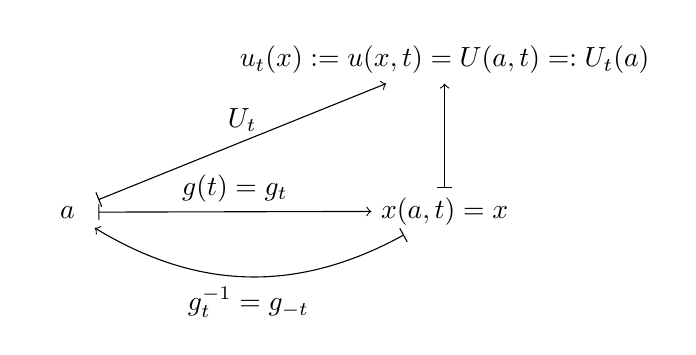
\begin{tikzpicture}
  \matrix (m) [matrix of math nodes, row sep=3.8em, column sep=4.8em, minimum width=2.2em]
  {
& u_t(x):= u(x,t) = U(a,t) =: U_t(a)    \\
    a  & x(a,t)=x   \\
};
  \path[|->]
  (m-2-1) edge node [above] {$U_t $} (m-1-2)
          edge node [above] {$g(t) = g_t$} (m-2-2)
  (m-2-2) edge node [auto]  {$$} (m-1-2)
          edge [bend left=30] node [below] {$g_t^{-1} = g_{-t}$} (m-2-1)
  ;
\end{tikzpicture}  







%\begin{figure}[b]
%  \centering
%  \includegraphics[width=\columnwidth]{../eps/Nielsen2011RBB_qualitative_report_topicsentiment}
%  \caption{Web service screenshot with text from Wikipedia
%    article ``Lundbeck''.}
%  \label{fig:topicsentiment}
%\end{figure}






\end{multicols*}

\begin{thebibliography}{9}

\bibitem{RBaierlein1999}
Ralph Baierlein. \textbf{Thermal Physics} Cambridge University Press (July 28, 1999), ISBN-13: 978-0521658386

\bibitem{CKittelHKroemer1980}
Charles Kittel, Herbert Kroemer, \textbf{Thermal Physics}, W. H. Freeman; Second Edition edition, 1980. 
ISBN-13: 978-0716710882

\bibitem{BSchutz1980}
Bernard F. Schutz, \textbf{Geometrical Methods of Mathematical Physics}, Cambridge University Press, 1980.
ISBN-13: 978-0521298872

\bibitem{CBorgnakkeRSonntag2012}
Claus Borgnakke, Richard E. Sonntag.  \textbf{Fundamentals of Thermodynamics}, 8th Edition, Wiley, (December 26, 2012). 
ISBN-13: 978-1118131992  

\end{thebibliography}
There is a Third Edition of T. Frankel's \textbf{The Geometry of Physics} \cite{TFrankel2004}, but I don't have the funds to purchase the book (about \$ 71 US dollars, with sales tax). It would be nice to have the hardcopy text to see new updates and to use for research, as the second edition allowed me to formulate fluid mechanics and elasticity in a covariant manner.  Please help me out and donate at \url{ernestyalumni.tilt.com}.  




\clearpage
\onecolumn

\section{Code listings}

\definecolor{darkgreen}{rgb}{0, 0.4, 0}
\lstset{language=Python,
  numbers=left,
  frame=bottomline,
  basicstyle=\scriptsize,
  identifierstyle=\color{blue},
  keywordstyle=\bfseries,
  commentstyle=\color{darkgreen},
  stringstyle=\color{red},
  literate={Ö}{{\"O}}1 {é}{{\'e}}1 {Å}{{\AA}}1,
}
\lstlistoflistings


%\label{listing:brede_str_nmf}\lstinputlisting{../../matlab/brede/python/brede_str_nmf}


\newpage
\section{Automatic generation of documentation}

Demontration using epydoc:
\begin{verbatim}
epydoc --pdf -o /home/fnielsen/tmp/epydoc/ --name RBBase wikipedia/api.py
\end{verbatim}
This example does not use \verb!brede_str_nmf! but another more
well-documented module called {\tt api.py} that are used to download
material from Wikipedia. 

%\includepdf[pages={-}]{/home/fnielsen/tmp/epydoc/api.pdf}

\end{document}
